\documentclass[10pt,t]{beamer}

\usepackage{listings}
\usepackage{bm}
\usepackage{amsmath}
\usepackage[utf8]{inputenc}

\def\figDir{figures}
\def\figDirLogos{figures/logos}
\def\figDirMacroIdent{figures/macro_identification}
\def\figDirMacroArtery{figures/macro_artery}
\def\figDirMacroHeart{figures/macro_heart}
\def\figDirMacroPerfusion{figures/macro_perfusion}
\def\figDirHomPerfusion{figures/homogenization_perfusion}
\def\figDirHomBones{figures/homogenization_bones}

\newcommand{\sfepy}{SfePy}
\newcommand{\isfepy}{\texttt{isfepy}}
\newcommand{\red}[1]{{\color{red}{#1}}}
\newcommand{\blue}[1]{{\color{blue}{#1}}}
\definecolor{lblue}{rgb}{0.0,0.4,1.0}
\newcommand{\lblue}[1]{{\color{lblue}{#1}}}
\definecolor{dgreen}{rgb}{0.0,0.4,0.11}
\newcommand{\dgreen}[1]{{\color{dgreen}{#1}}}

\def \pder#1#2{\frac{\partial #1}{\partial #2}}
%\newcommand{\dvg}{\mathop{\rm div}}
\newcommand{\grad}{\mathop{\rm grad}}
\newcommand{\ul}[1]{\underline{#1}}
\def\half{{\textstyle{1\over2}}}
\def\d{{\rm d}}

\newcommand{\bmi}[1]{\textbf{\textit{#1}}}
\def\sigmabf{\bm{\sigma}}
\def\ub{{\bmi{u}}}
\def\nb{{\bmi{n}}}
\def\Db{{\bmi{D}}}
\def\gb{{\bmi{g}}}
\def\Ccal{\mathcal{C}}
\def\mic{{\rm mic}}
\newcommand{\pd}{\partial}
\newcommand{\Om}{\Omega}
\newcommand{\om}{\omega}
\newcommand{\lam}{\lambda}
\newcommand{\veps}{\varepsilon}
\newcommand{\vphi}{\varphi}
\def\phibf{{\mbox{\boldmath$\varphi$\unboldmath}}}
\def\xibf{{\mbox{\boldmath$\xi$\unboldmath}}}
\newcommand{\smatrix}[2]{\left#2\begin{array}{#1}}
\newcommand{\ematrix}[1]{\end{array}\right#1}

%%
% Beamer related packages & defs.
\usepackage{multimedia}

\DeclareGraphicsExtensions{.pdf,.png,.jpg}

\mode<handout>{\beamertemplatesolidbackgroundcolor{black!5}}
\mode<presentation>
{
%  \usetheme{Frankfurt}
  \useoutertheme[subsection=false]{smoothbars}
  \setbeamerfont{block title}{size={}}
  \usefonttheme[onlymath]{serif}
%  \useinnertheme{rectangles}
%  \useinnertheme[shadow=true]{rounded}
  \useinnertheme{rounded}
%  \useinnertheme{circles}
%  \useinnertheme{inmargin}
  \setbeamercovered{transparent}
  \usecolortheme{seahorse}
  \usecolortheme{rose}
%  \beamertemplategridbackground[0.2cm]
  \beamertemplatetransparentcovereddynamic

  \setbeamertemplate{navigation symbols}{
%    \insertdocnavigationsymbol
%    \insertsubsectionnavigationsymbol 
    \insertbackfindforwardnavigationsymbol
    \hspace{1mm} \hbox{\normalsize \insertframenumber/\inserttotalframenumber}
  }
}

\bibliographystyle{plain}

\title{What we do in Biomechanics}

\author{Robert Cimrman \& Eduard Rohan \& \dots}

\institute%[University of West Bohemia]
{
  Department of Mechanics \& New Technologies Research Centre \\
  University of West Bohemia in Plze\v{n}, Czech Republic
}

%
\titlegraphic{
\begin{tabular}{lcr}
  
\includegraphics[height=1.0cm]{\figDirLogos/logo_zcu} &
  
\includegraphics[height=1.0cm]{\figDirLogos/logo_ntc_en_i} &
  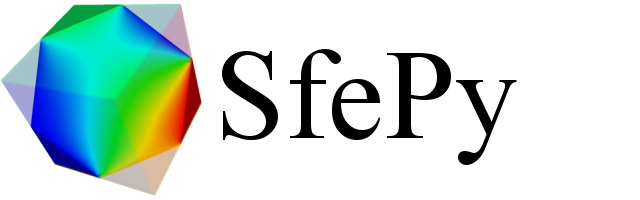
\includegraphics[height=1.0cm]{\figDirLogos/sfepy_logo_title}
\end{tabular}
}
%


\begin{document}

\frame{\titlepage}

\begin{frame}
  \frametitle{Outline}
  \tableofcontents
\end{frame}

\section{Macroscopic Models}

\subsection{Soft Tissue Models: Parameter Identification}

\begin{frame}
  \frametitle{Soft Tissue Models:  Parameter Identification}
  \begin{itemize}
  \item complex soft tissue models
    \begin{itemize}
    \item smooth, skeletal, or cardiac muscles
    \item large deformations
    \end{itemize}
  \item mixture of the extracellular \emph{matrix} and muscle \emph{fibres}
  \item \emph{automatic identification algorithm}
    \begin{itemize}
    \item many constitutive parameters to identify from \emph{measurements}
    \end{itemize}
  \end{itemize}
  \begin{center}
    \begin{minipage}{0.35\linewidth}
      \scriptsize
      quantitative microscopy \\
      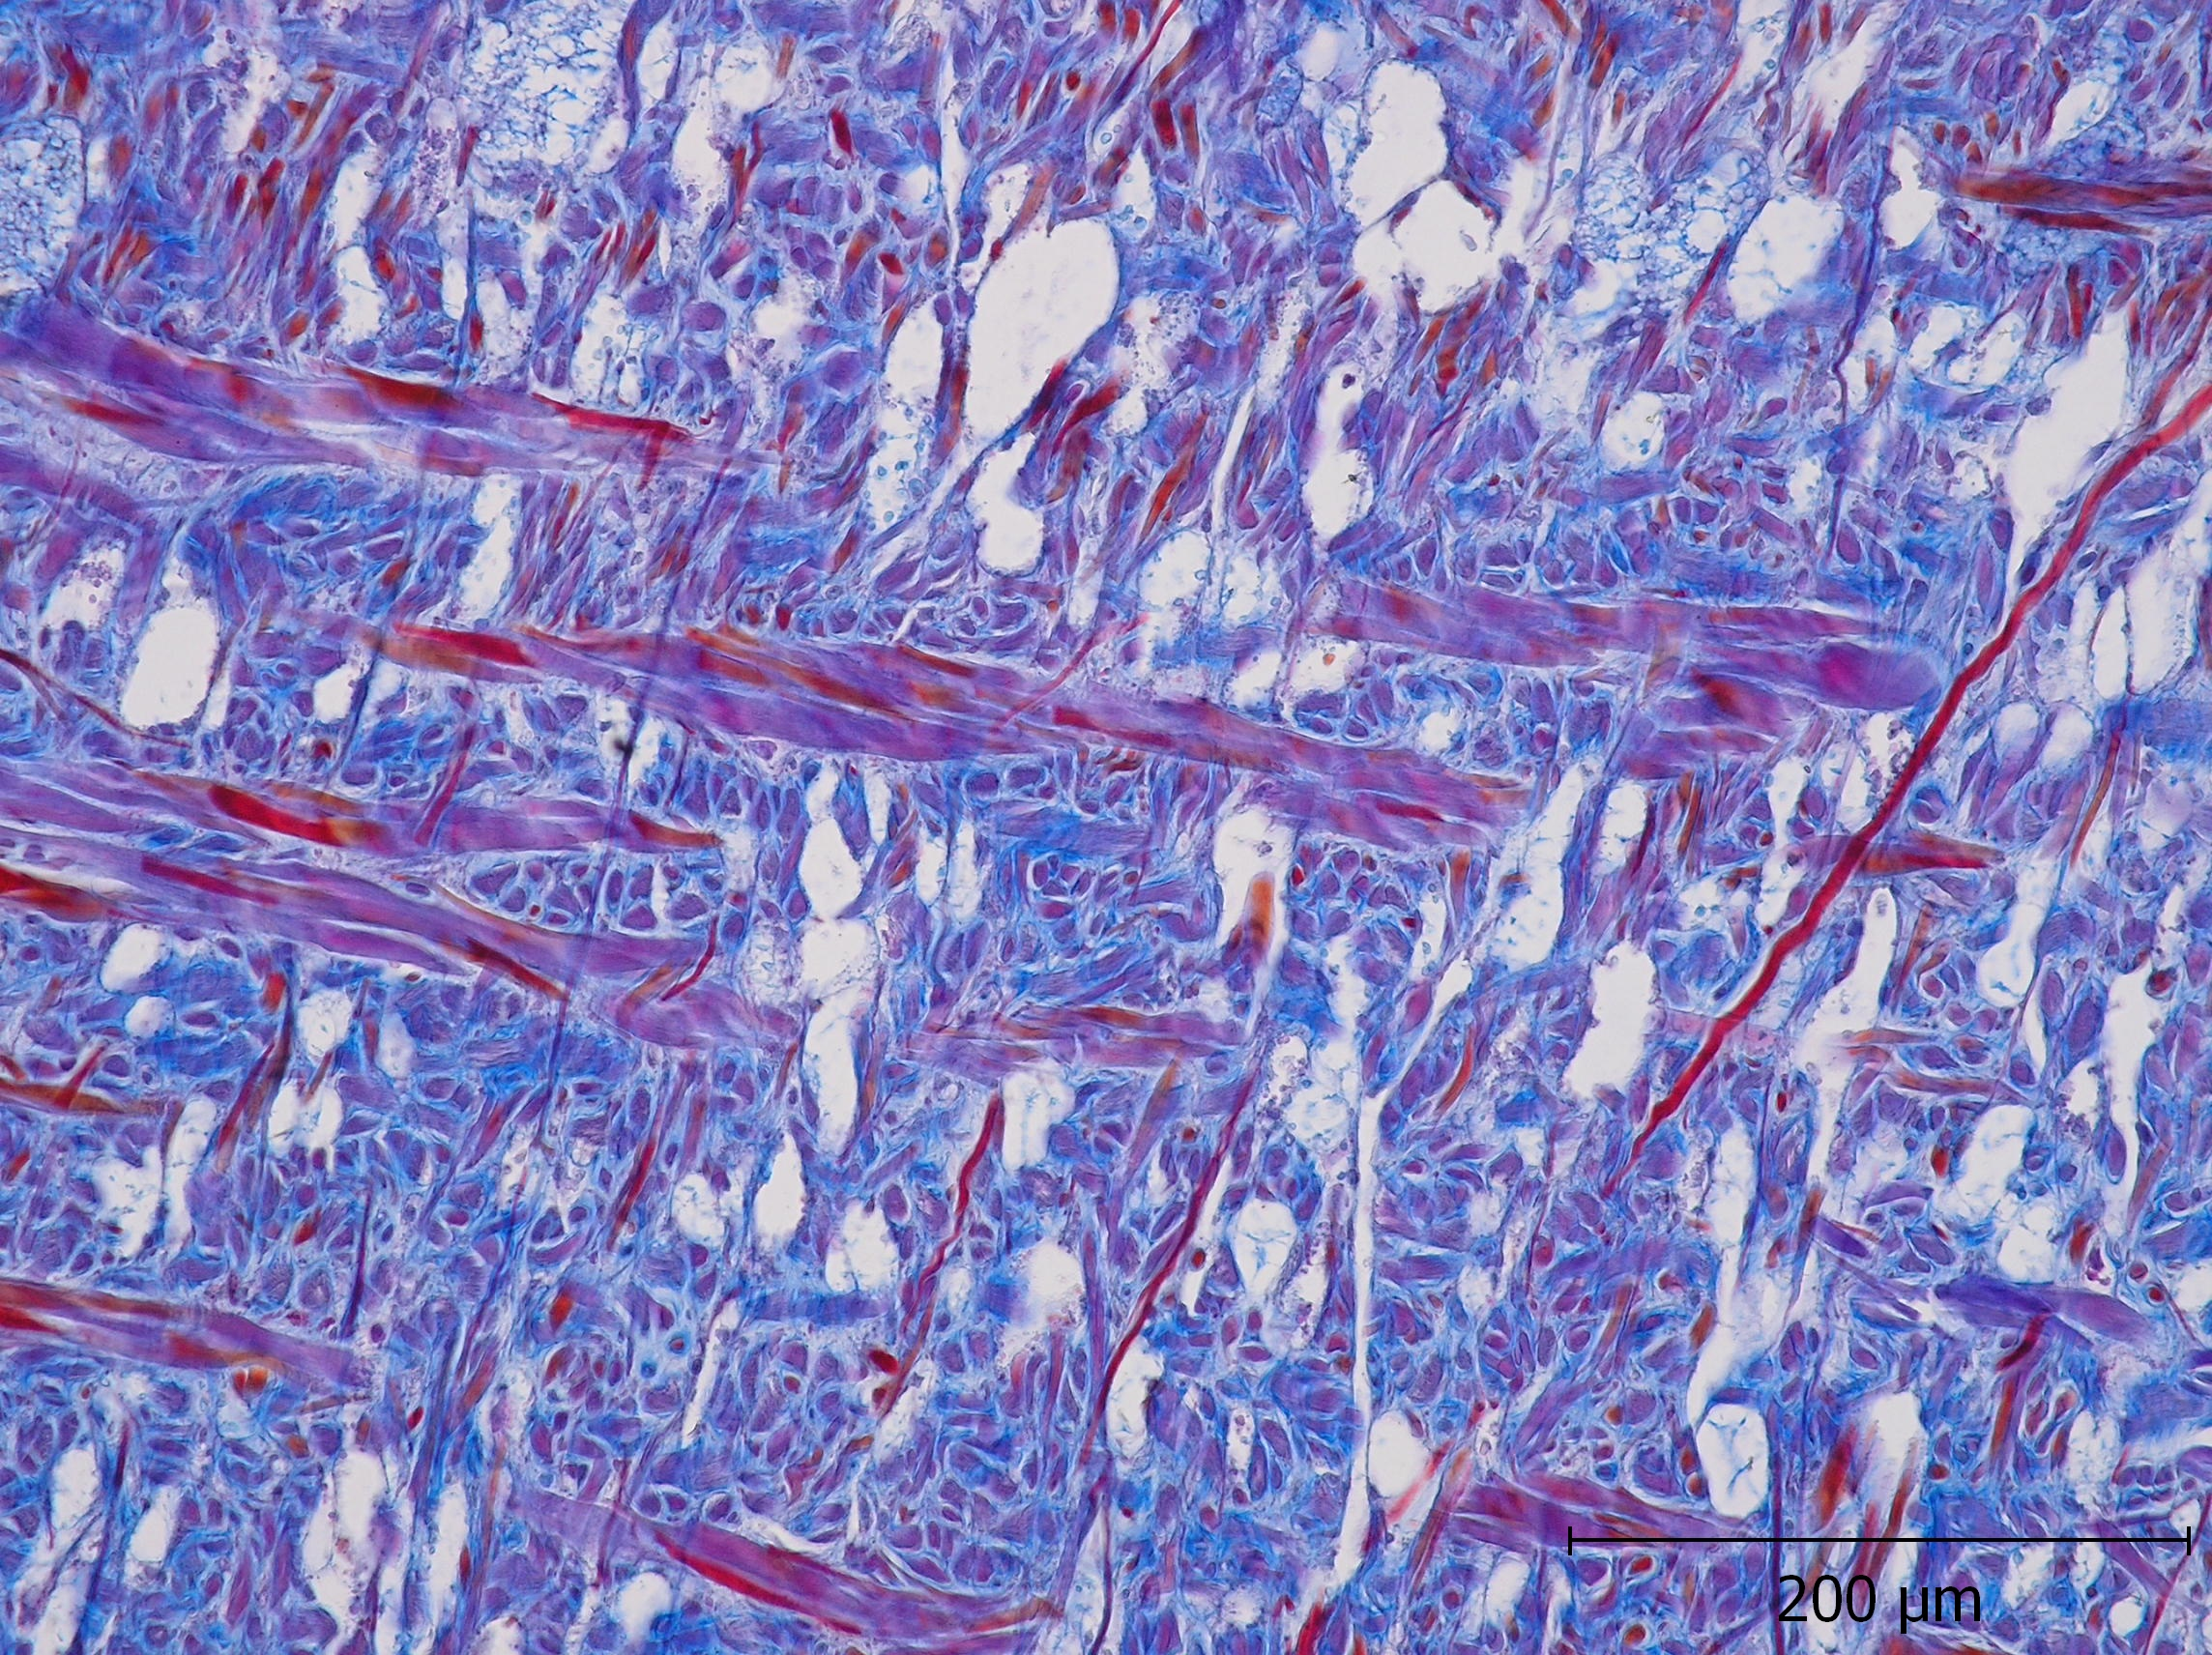
\includegraphics[width=\linewidth]{\figDirMacroIdent/51_04_02a}
    \end{minipage}
    \hfill
    \begin{minipage}{0.28\linewidth}
      \scriptsize
      finite element modeling \\
      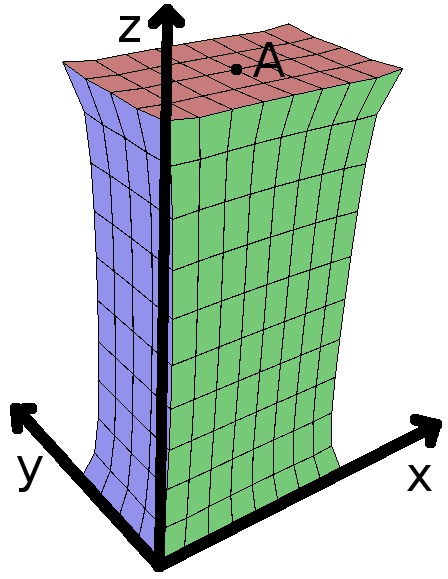
\includegraphics[width=0.8\linewidth]{\figDirMacroIdent/finaldef}
    \end{minipage}
    \hfill
    \begin{minipage}{0.35\linewidth}
      \scriptsize
      fit to measured data \\
      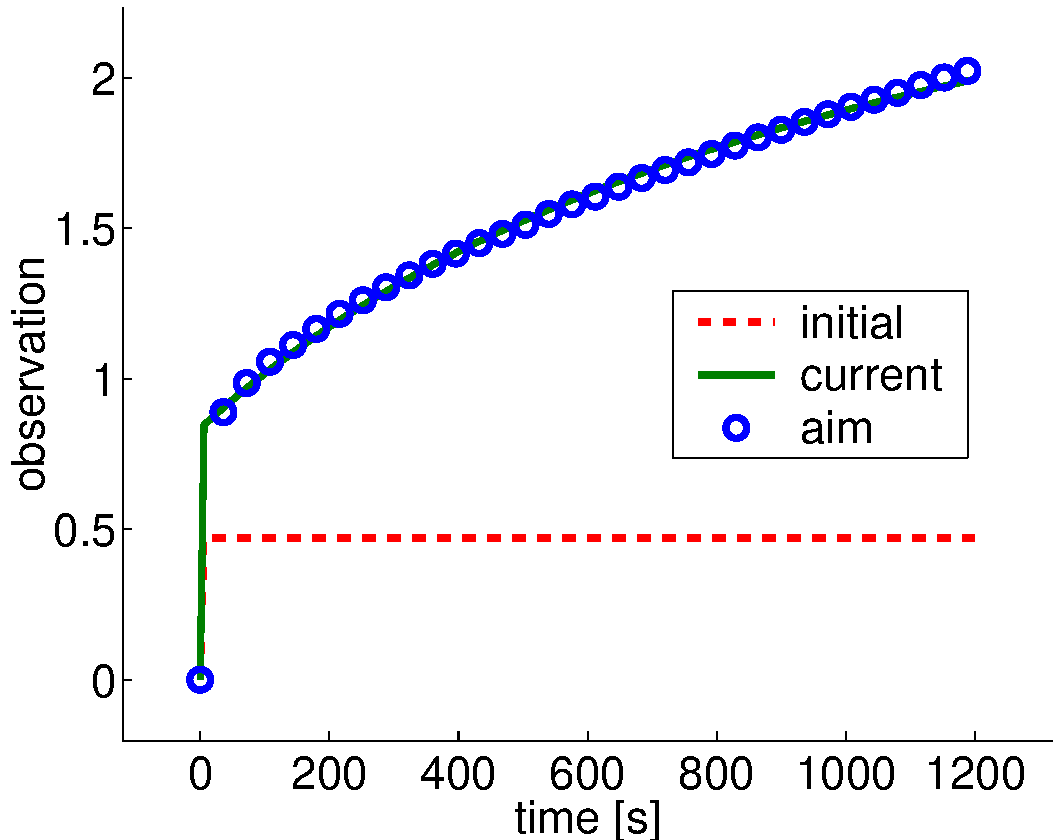
\includegraphics[width=\linewidth]{\figDirMacroIdent/saConv0022}
    \end{minipage}
  \end{center}
\end{frame}


\subsection{Macroscopic Arterial Wall Modeling}

\begin{frame}
  \frametitle{Macroscopic Arterial Wall Modeling}
  \begin{itemize}
  \item \emph{composite model} of smooth muscle tissue
    \begin{itemize}
    \item matrix, elastin, collagen fibres
    \item $2^{nd}$ Piola-Kirchhoff stress:
      \begin{equation}
        \label{eq:2pk}
        S_{ij} = - J C_{ij}^{-1}p + \phi_m \frac{\partial W^m}{\partial E_{ij}}
        + \phi_e \tau_{ij}^e + \phi_c \tau_{ij}^c
      \end{equation}
    \end{itemize}
  \item assessing \emph{aneurysms} in abdominal aorta
    \begin{itemize}
    \item parametric study: changing aneurysm geometry
    \end{itemize}
  \end{itemize}
  \begin{center}
    \begin{minipage}{0.28\linewidth}
      \scriptsize
      orientation of fibres \\
      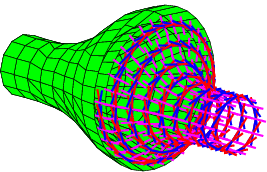
\includegraphics[width=\linewidth]{\figDirMacroArtery/0mesh_fibr_AAA}
    \end{minipage}
    \hfill
    \begin{minipage}{0.4\linewidth}
      \scriptsize
      aneurysm geometry \\
      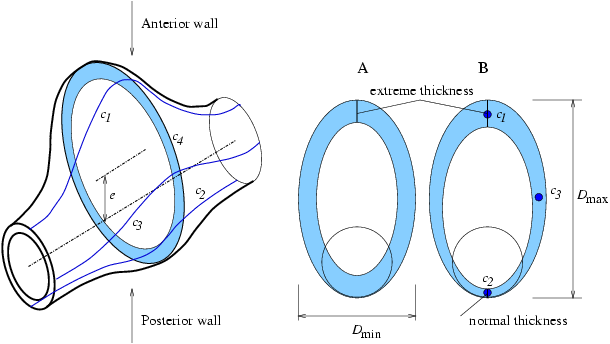
\includegraphics[width=0.9\linewidth]{\figDirMacroArtery/AAA_scheme}
    \end{minipage}
    \hfill
    \begin{minipage}{0.28\linewidth}
      \scriptsize
      stress in elastin fibres \\
      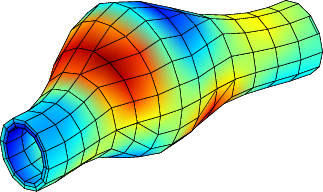
\includegraphics[width=0.8\linewidth]{\figDirMacroArtery/aaa01_2} \\
      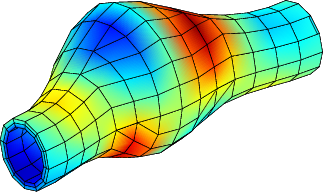
\includegraphics[width=0.8\linewidth]{\figDirMacroArtery/aaa01_3}
    \end{minipage}
  \end{center}
\end{frame}


\subsection{Heart Modeling}

\begin{frame}
  \frametitle{Heart Modeling}
  \begin{itemize}
  \item modeling \emph{pathologies}: e.g. ischemic heart
  \item parameter identification from displacements, pressure measurements
  \item output: \emph{global indicators} of beating heart: blood pressure,
    ejection volume
  \item in collaboration with INRIA Rocquencourt, France (Jacques Sainte-Marie,
    Dominique Chapelle and others)
  \end{itemize}
  \begin{center}
    \begin{minipage}{0.28\linewidth}
      \scriptsize
      action potential \\
      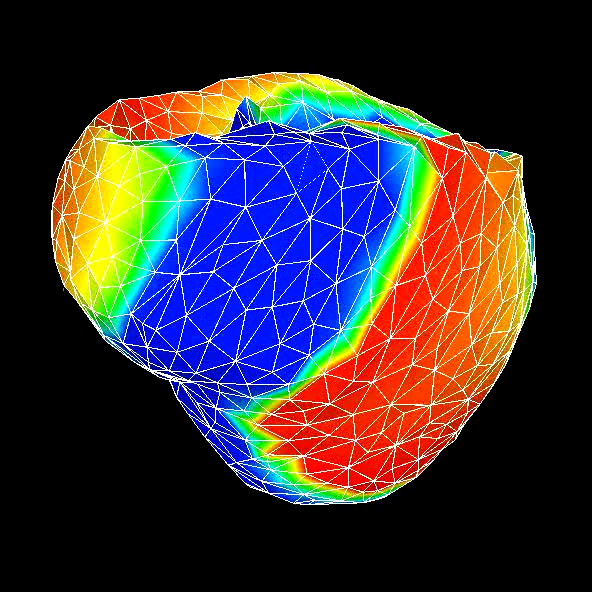
\includegraphics[width=0.9\linewidth]{\figDirMacroHeart/activ1}
    \end{minipage}
    \hfill
    \begin{minipage}{0.4\linewidth}
      \scriptsize
      global indicators: healthy (dashed) and ischemic (solid) heart \\
      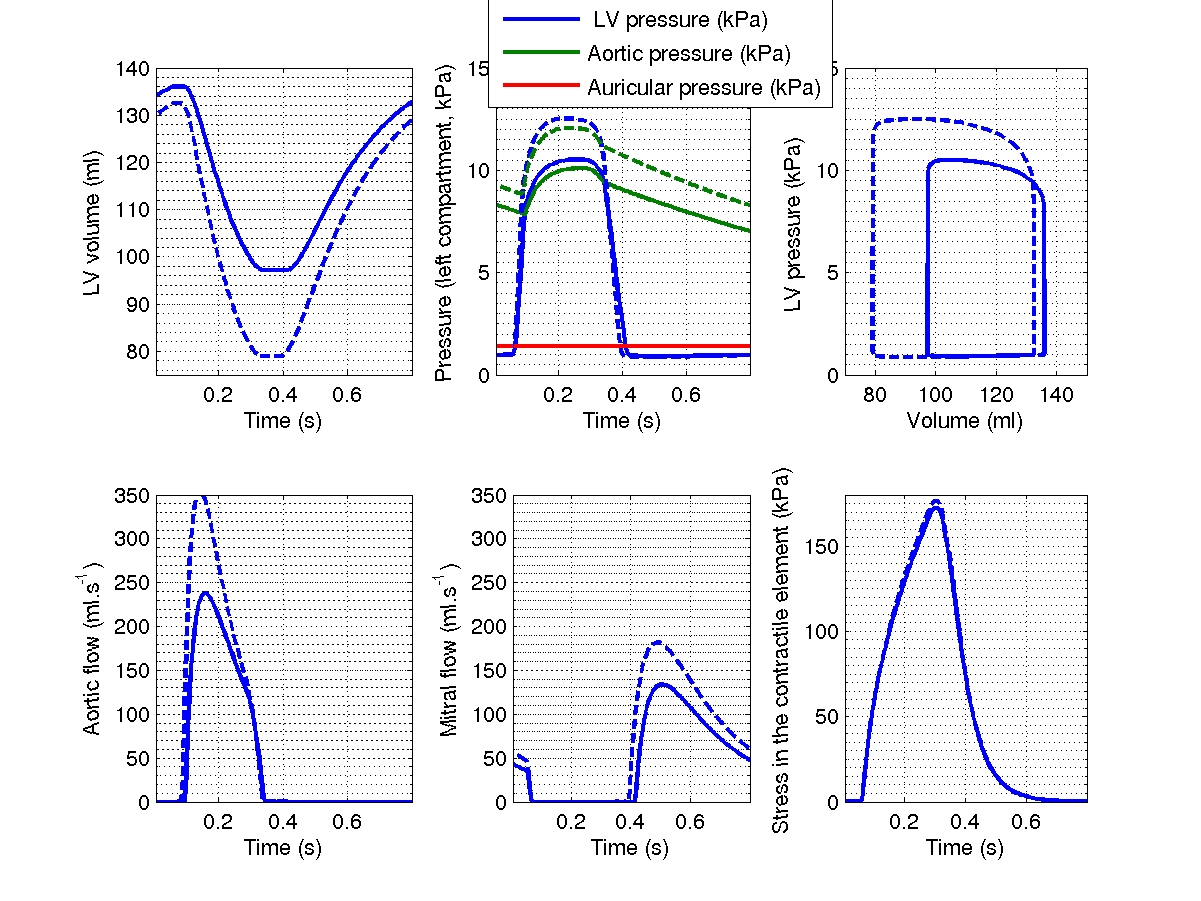
\includegraphics[width=\linewidth]{\figDirMacroHeart/compar_u1}
    \end{minipage}
    \hfill
    \begin{minipage}{0.28\linewidth}
      \scriptsize
      stress in ischemic heart \\
      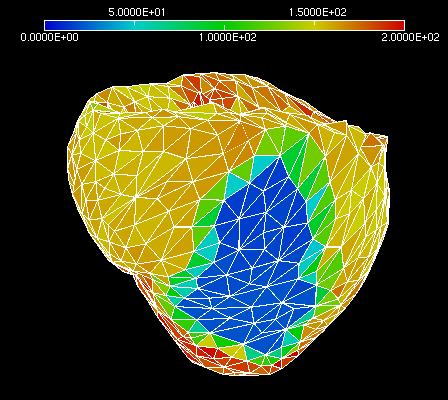
\includegraphics[width=0.9\linewidth]{\figDirMacroHeart/stress_path}
    \end{minipage}
  \end{center}
\end{frame}


\subsection{Perfused Muscle Tissue: Heart, Kidneys}

\begin{frame}
  \frametitle{Perfused Muscle Tissue: Heart, Kidneys}
  \begin{itemize}
  \item \emph{solid--fluid mixture}, large content of water, but almost solid
    \dots
  \item transport in soft tissue
    \begin{itemize}
    \item nutrient supply / drainage of waste
    \item transport of oxygen
    \item transport of ions  
    \end{itemize}
  \item coupling = feedback
    \begin{itemize}
    \item perfusion $\rightarrow$ muscular activity, contraction
      $\rightarrow$ perfusion
    \end{itemize}
  \end{itemize}
  \begin{center}
    \begin{minipage}{0.28\linewidth}
      \scriptsize
      multiple channel systems \\
      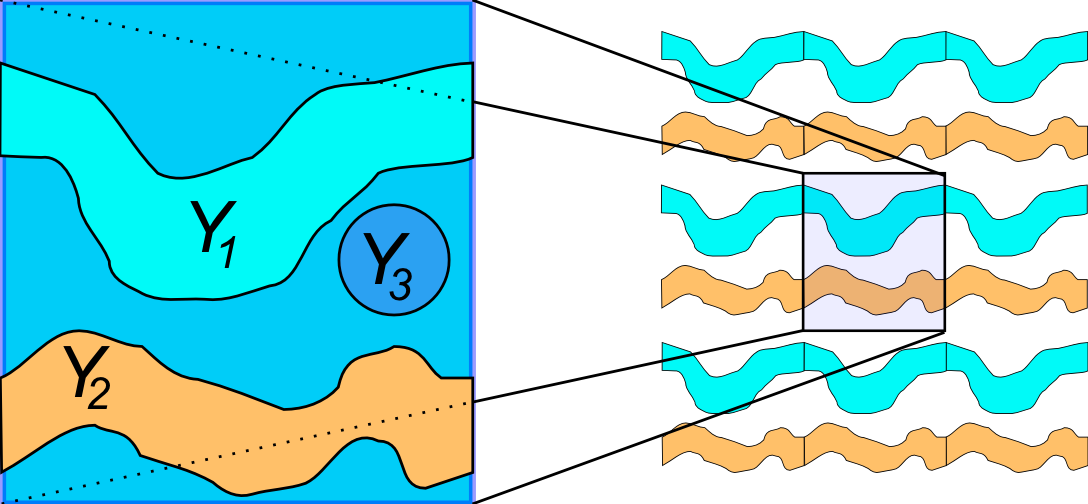
\includegraphics[width=0.9\linewidth]
      {\figDirMacroPerfusion/fig_2porous_Y-domain_new} \\

      \red{heart}: \\ $p_1$ arterial, $p_2$ venous pressure
      $p_v$ ventricular pressure traction

      \blue{kidneys}: \\ $p_1$ arterial, $p_2$ venous, $p_3$ filtrate pressure
      $p_{\rm abd}$ abdominal pressure traction
    \end{minipage}
    \hfill
    \begin{minipage}{0.35\linewidth}
      \scriptsize
      application: heart \\
      \centering
      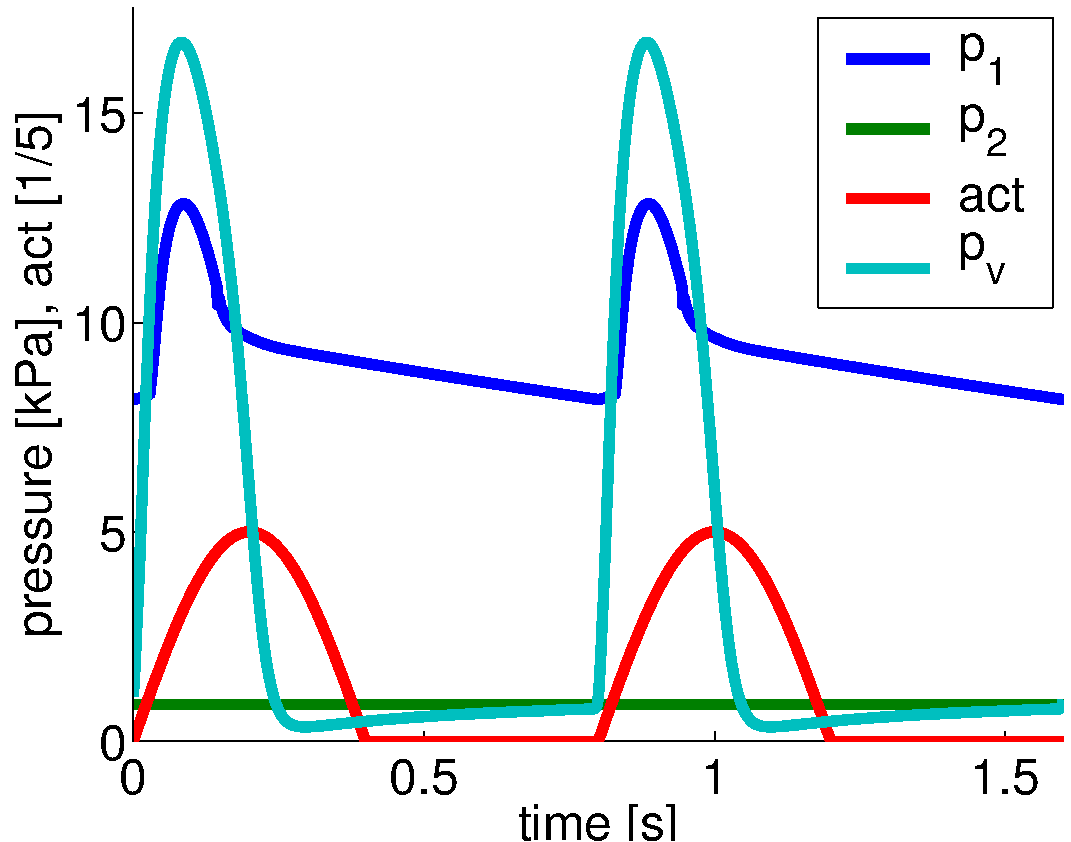
\includegraphics[width=0.6\linewidth]
      {\figDirMacroPerfusion/loads_heart} \\
      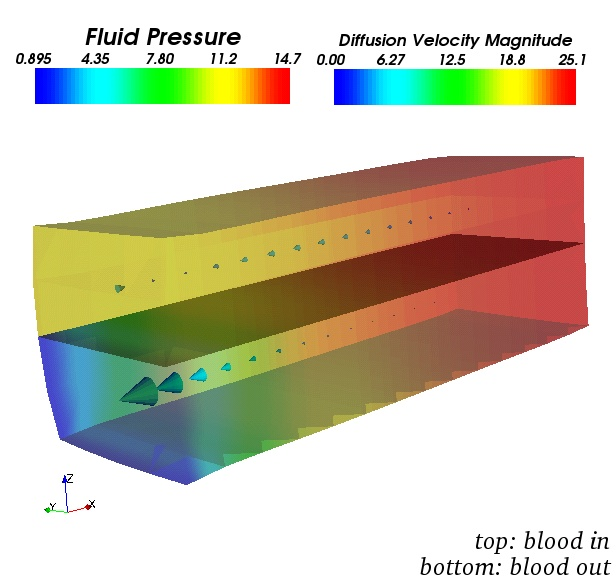
\includegraphics[width=0.6\linewidth]
      {\figDirMacroPerfusion/perfusion_heart_block_4_0026}
    \end{minipage}
    \hfill
    \begin{minipage}{0.35\linewidth}
      \scriptsize
      application: kidneys \\
      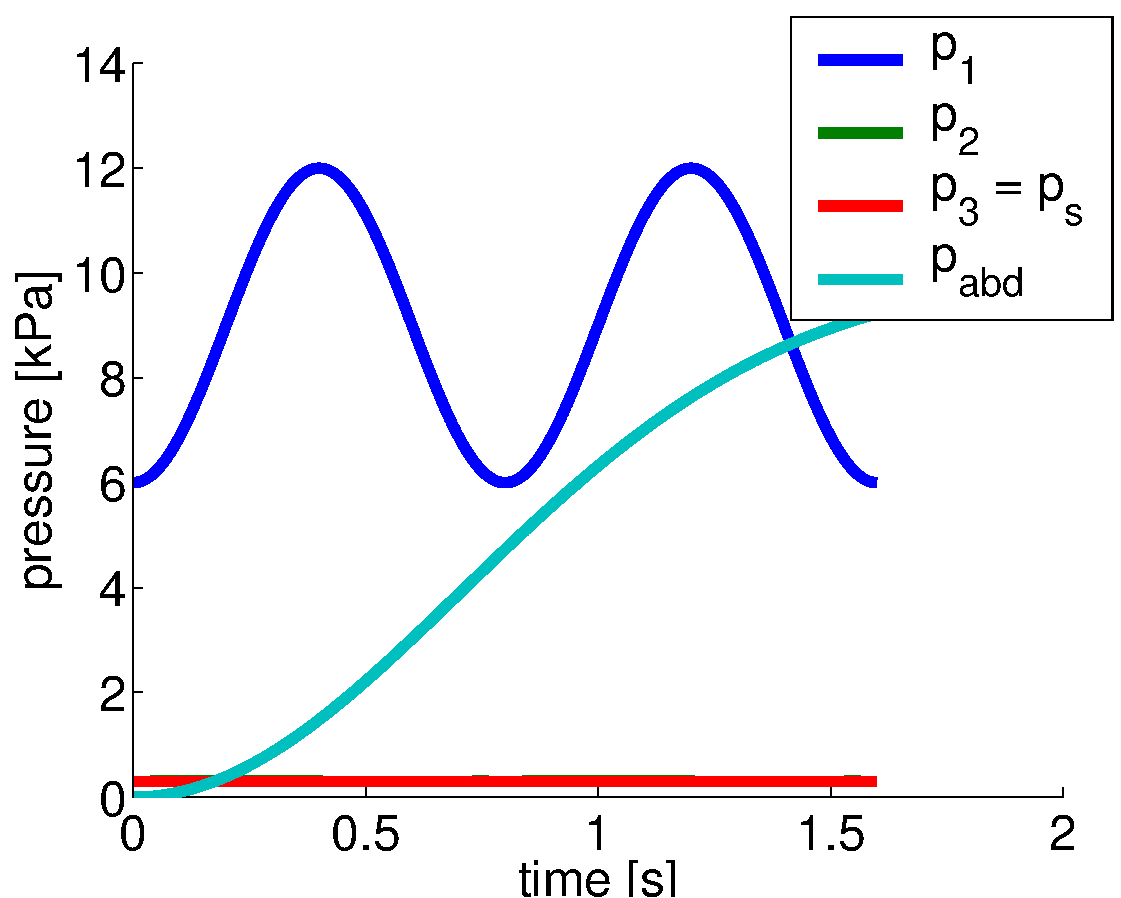
\includegraphics[width=0.6\linewidth]
      {\figDirMacroPerfusion/loads_kidney} \\
      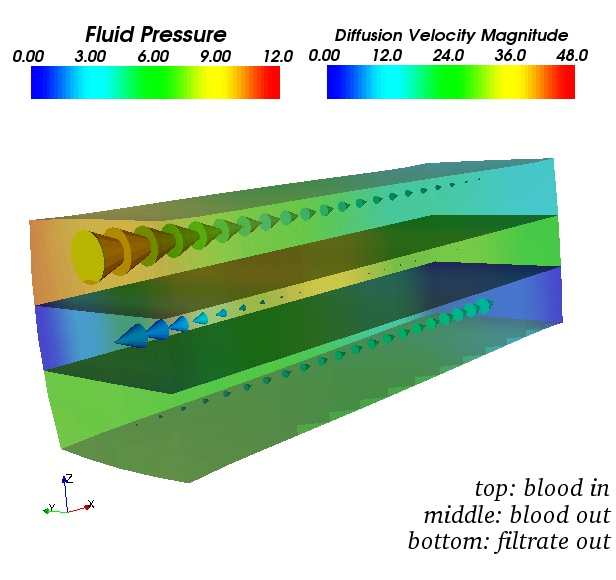
\includegraphics[width=0.6\linewidth]
      {\figDirMacroPerfusion/perfusion_kidney_block_3_0055}
    \end{minipage}
  \end{center}
\end{frame}


\section{Multiscale Models}

\subsection{Porous Media: Current Approach}

\begin{frame}
  \frametitle{Porous Media: Current Approach}
  \begin{itemize}
  \item treated by the theory of homogenization
    \centerline{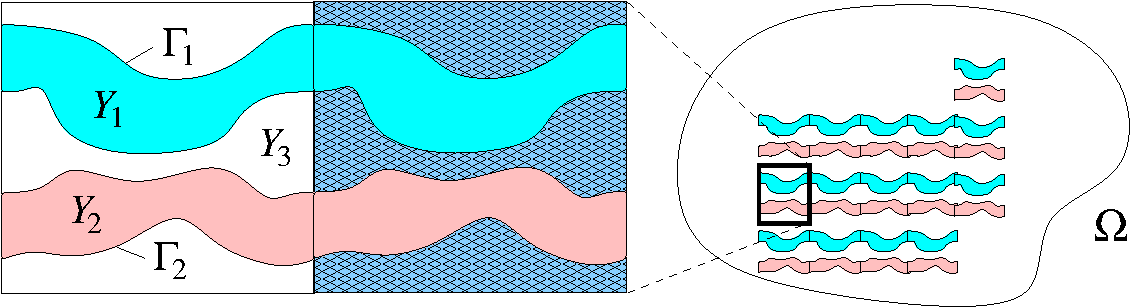
\includegraphics[width=0.6\linewidth]
      {\figDirHomPerfusion/fig_2porous_Y-domain-new-hsm}}
  \item modeling \emph{blood perfusion} in muscles, brain
  \item compact \emph{bone poromechanics}
  \item fading memory effects, \emph{stress recovery} at micro-level
  \end{itemize}
  \begin{center}
    \begin{minipage}[t]{0.6\linewidth}
      \scriptsize
      microstructure: two channels + porous matrix
      \begin{center}
        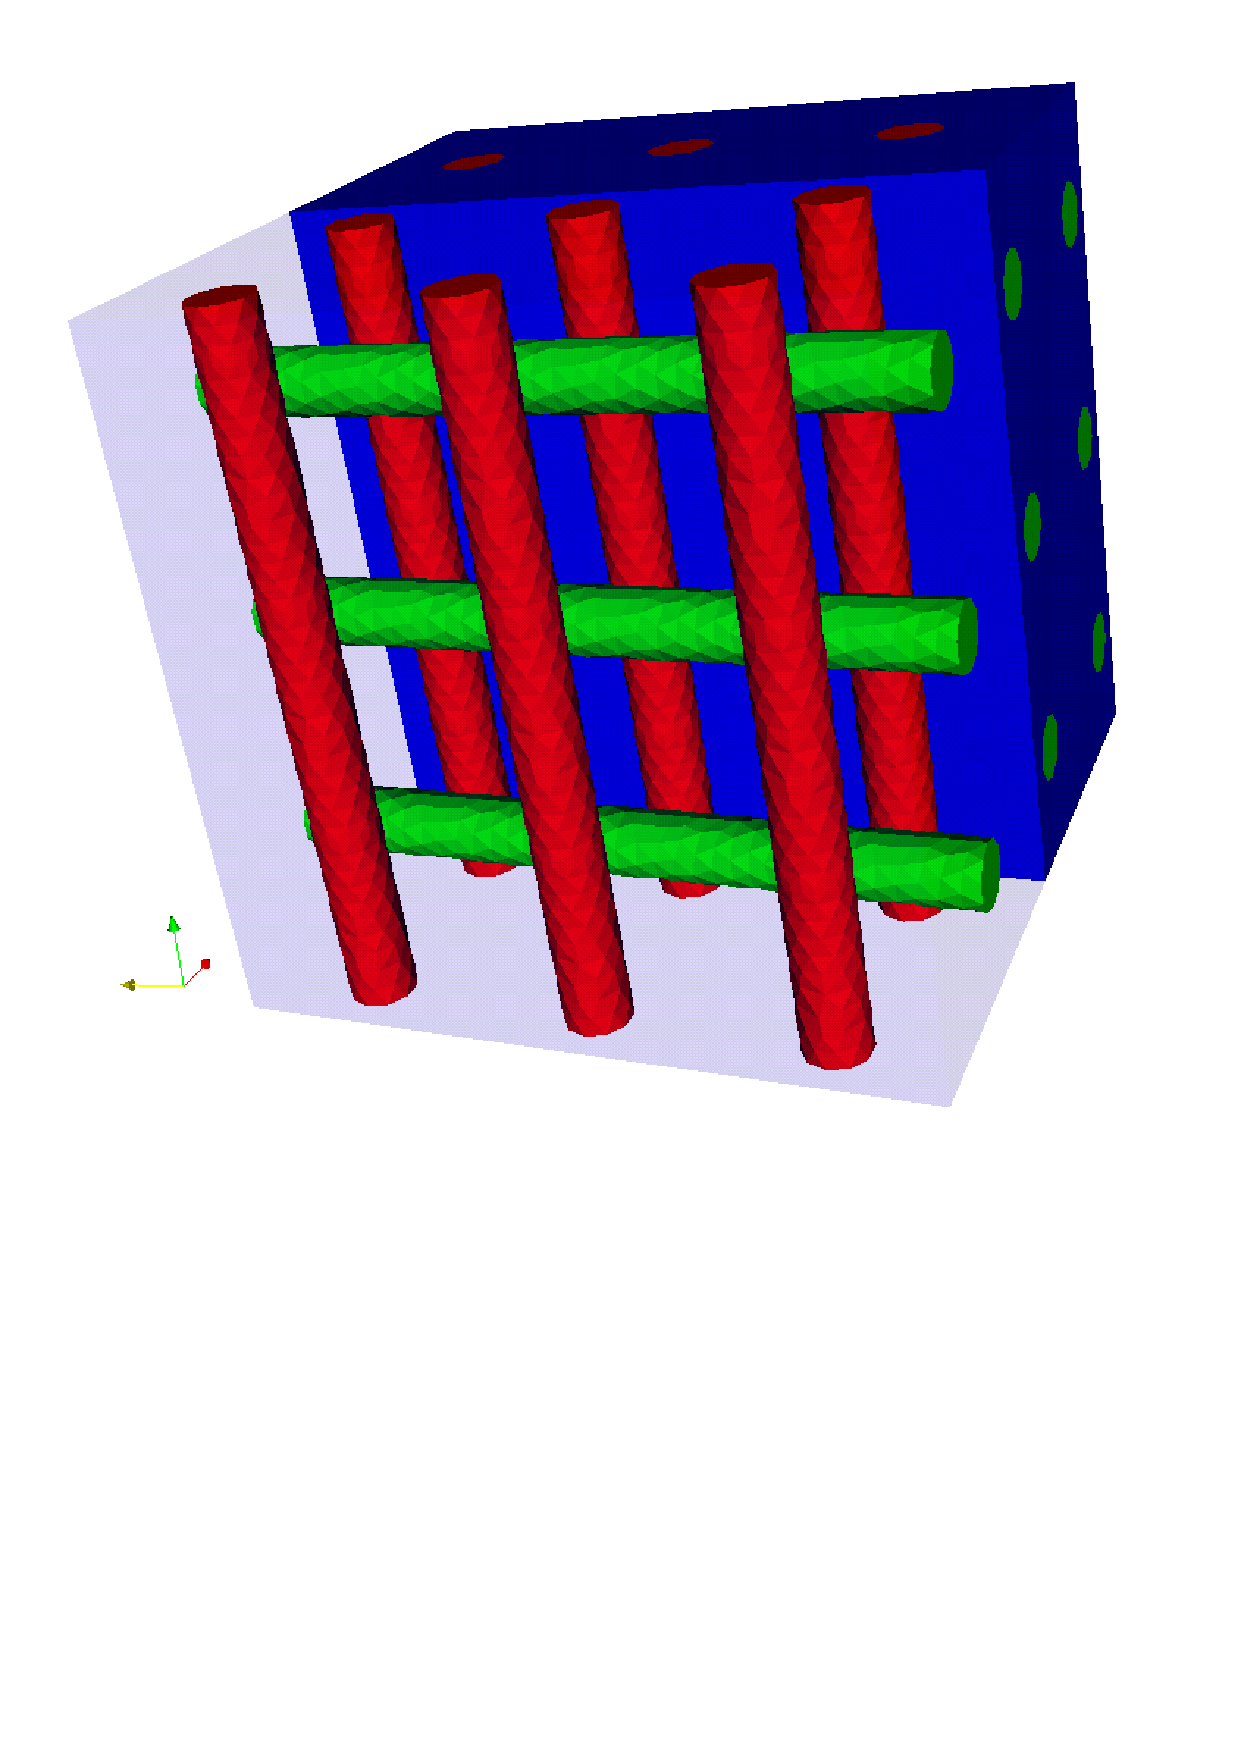
\includegraphics[width=0.5\linewidth]{\figDirHomPerfusion/micro_3d_M1}
        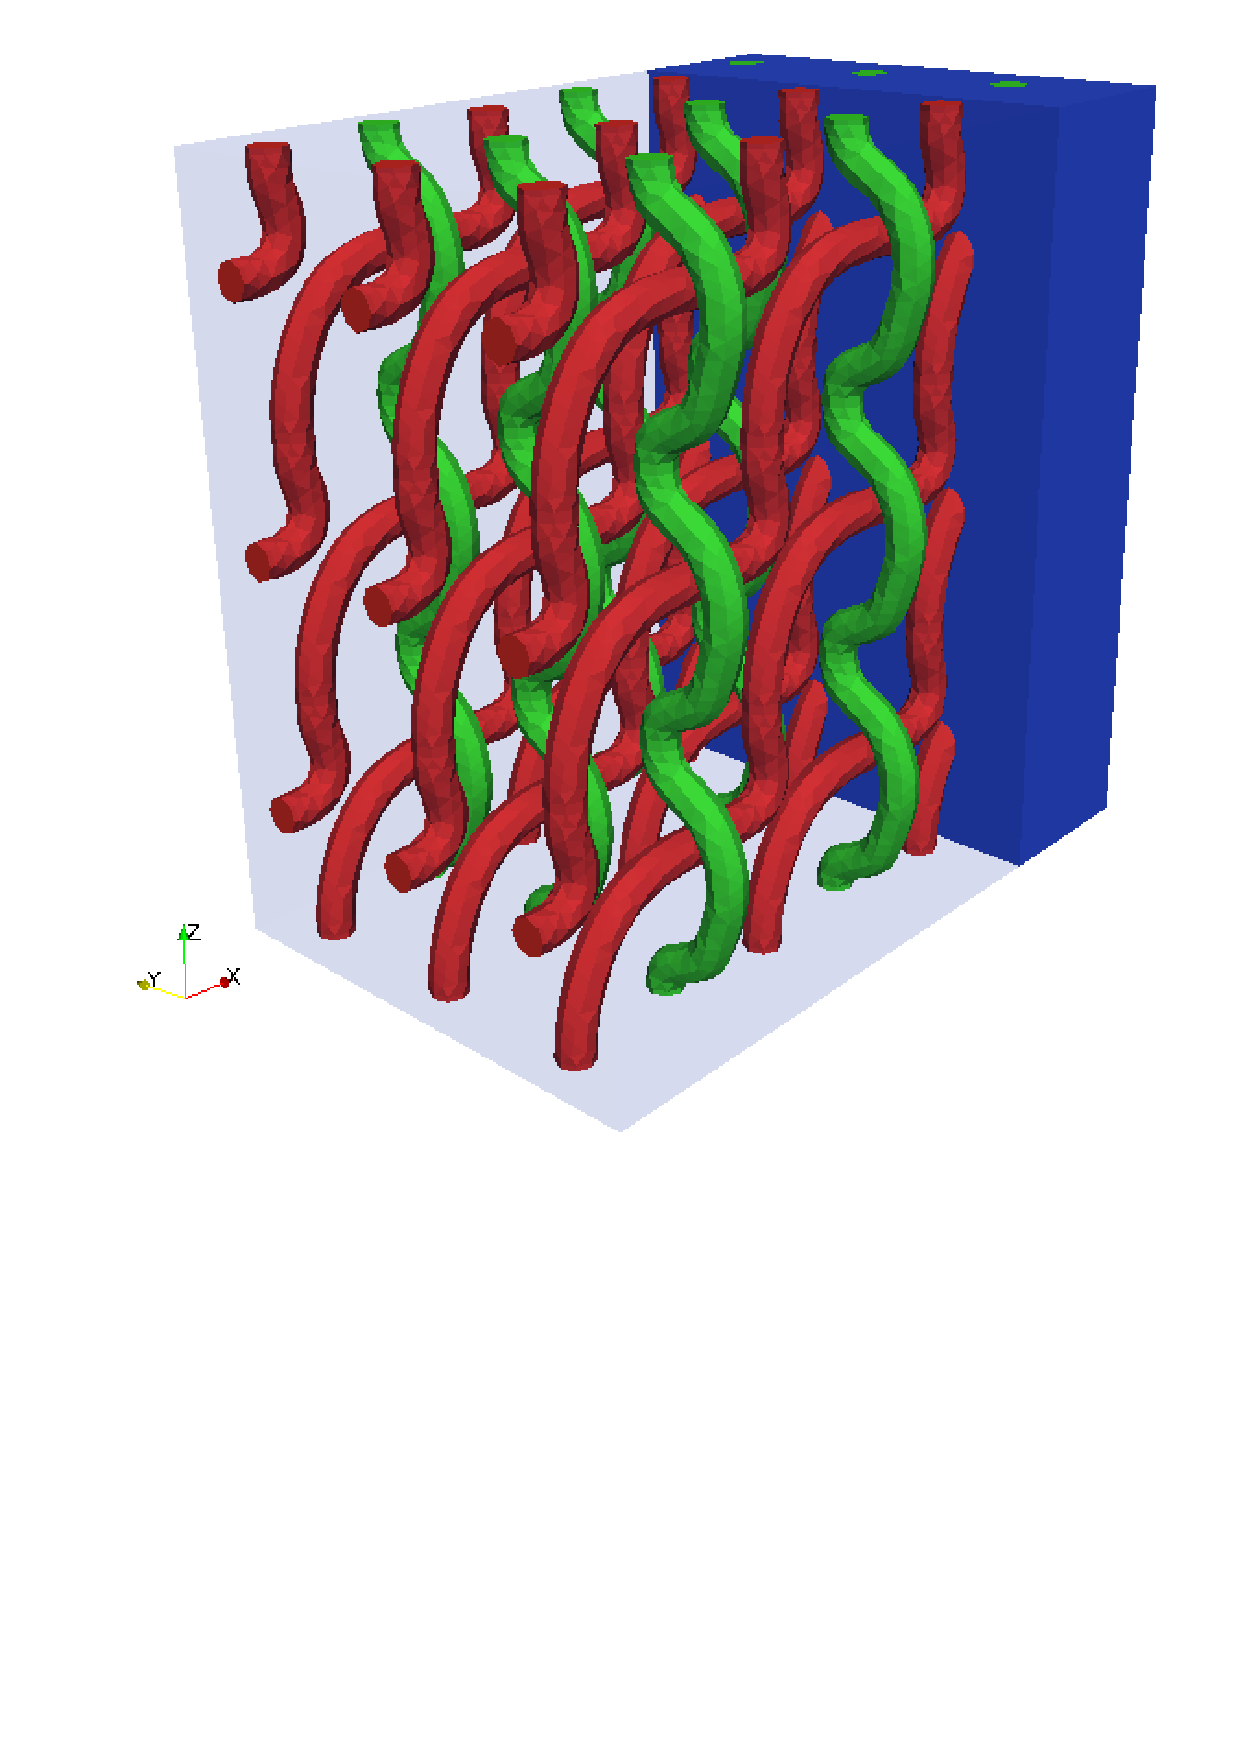
\includegraphics[width=0.5\linewidth]{\figDirHomPerfusion/micro_3d_M2}
      \end{center}
    \end{minipage}
    \hfill
    \begin{minipage}[t]{0.32\linewidth}
      \scriptsize
      microscopic corrector functions
      \begin{center}
        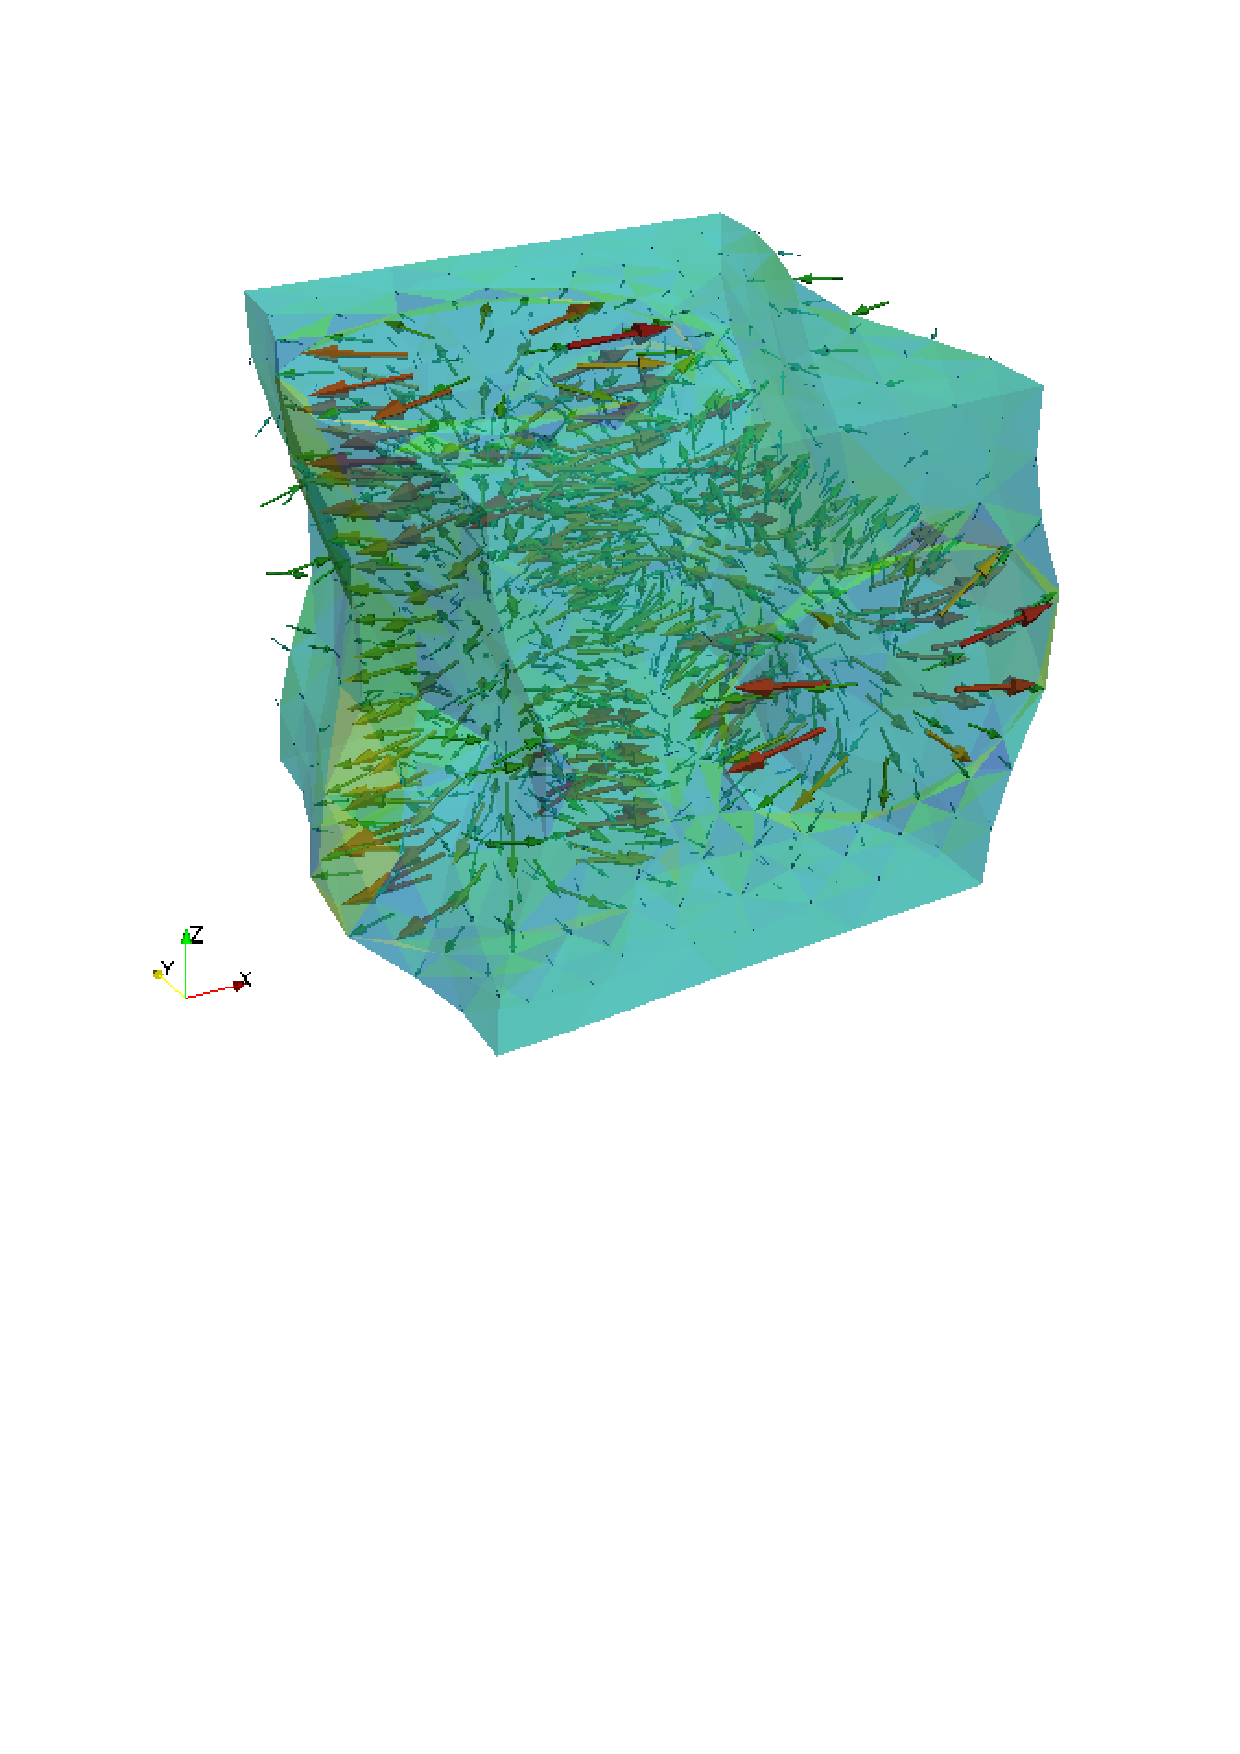
\includegraphics[width=0.5\linewidth]
        {\figDirHomPerfusion/steady_rs_00_u_M1_2}
        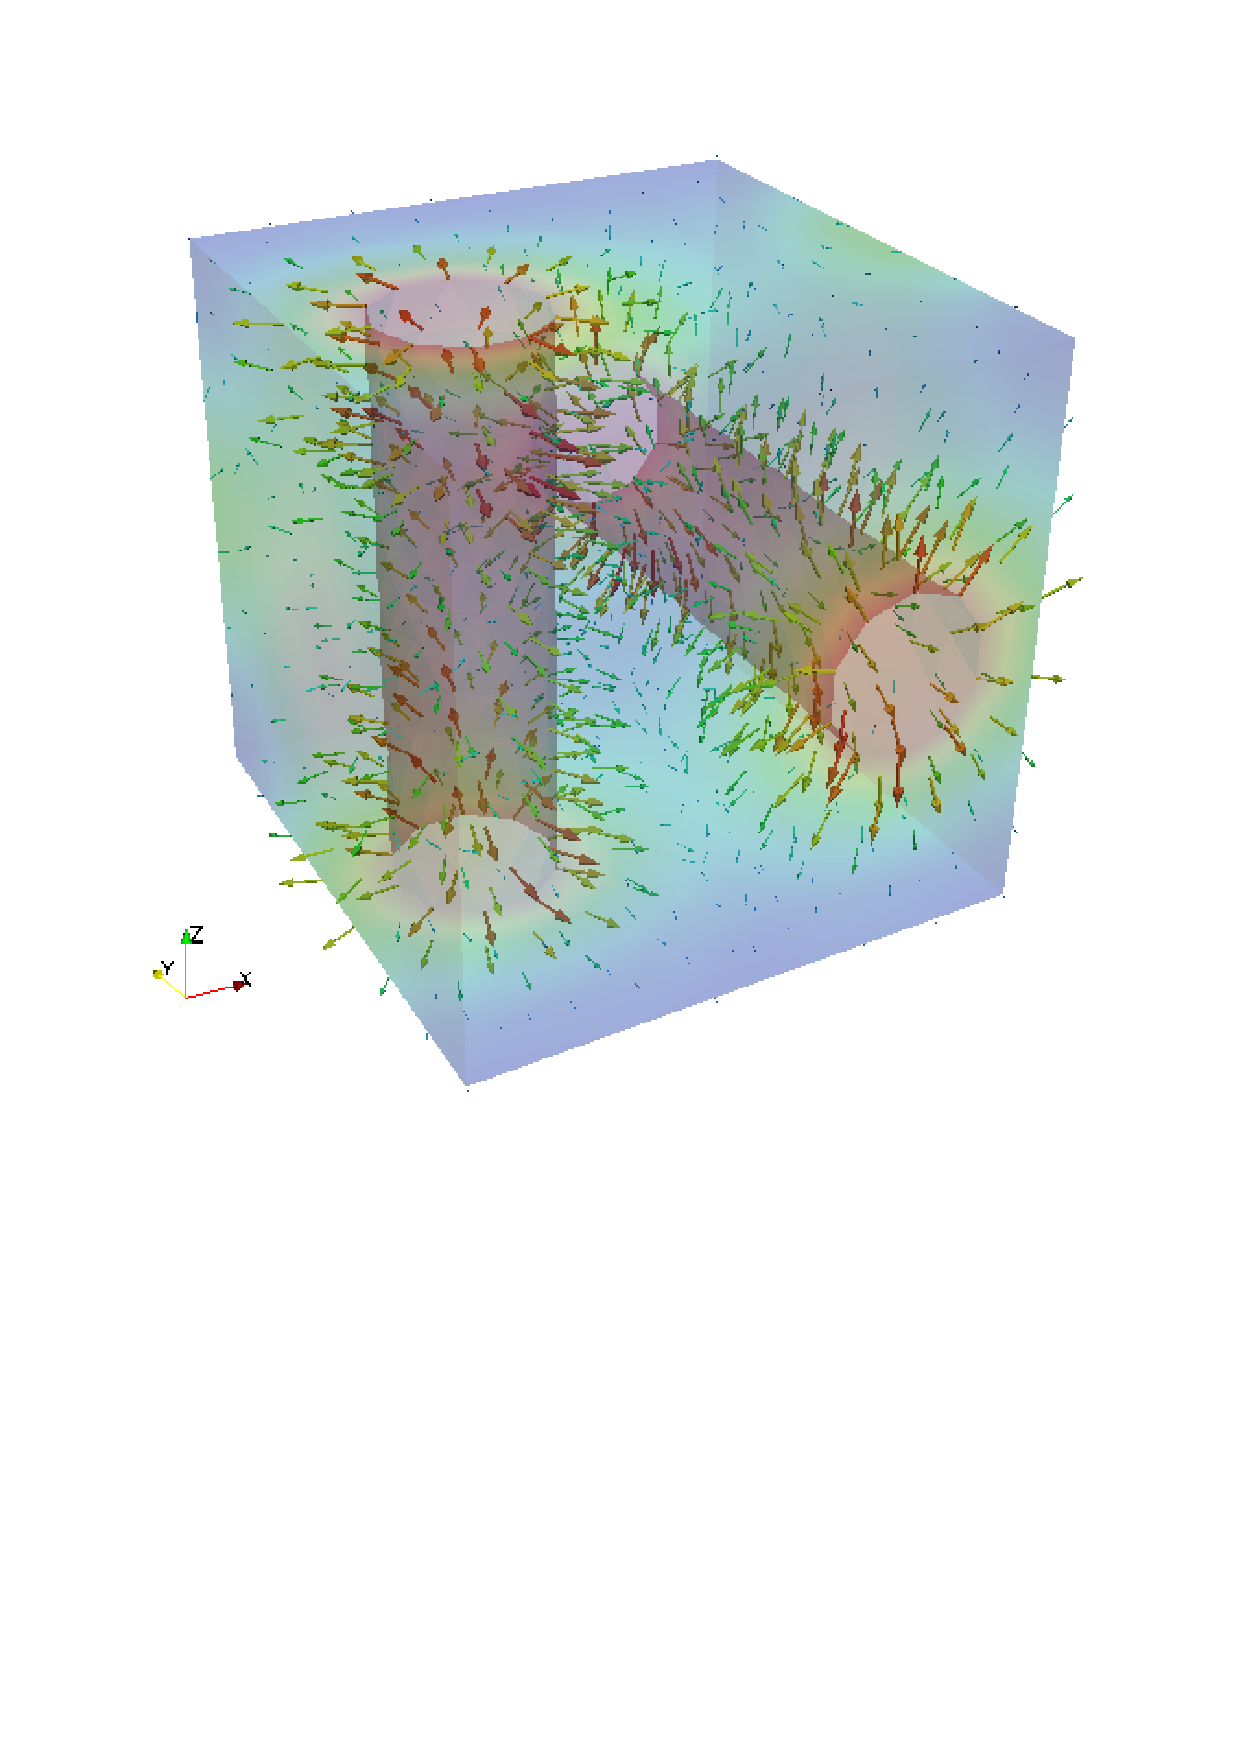
\includegraphics[width=0.5\linewidth]
        {\figDirHomPerfusion/steady_rs_00_p_M1_2} \\
        \vspace*{-10mm}
        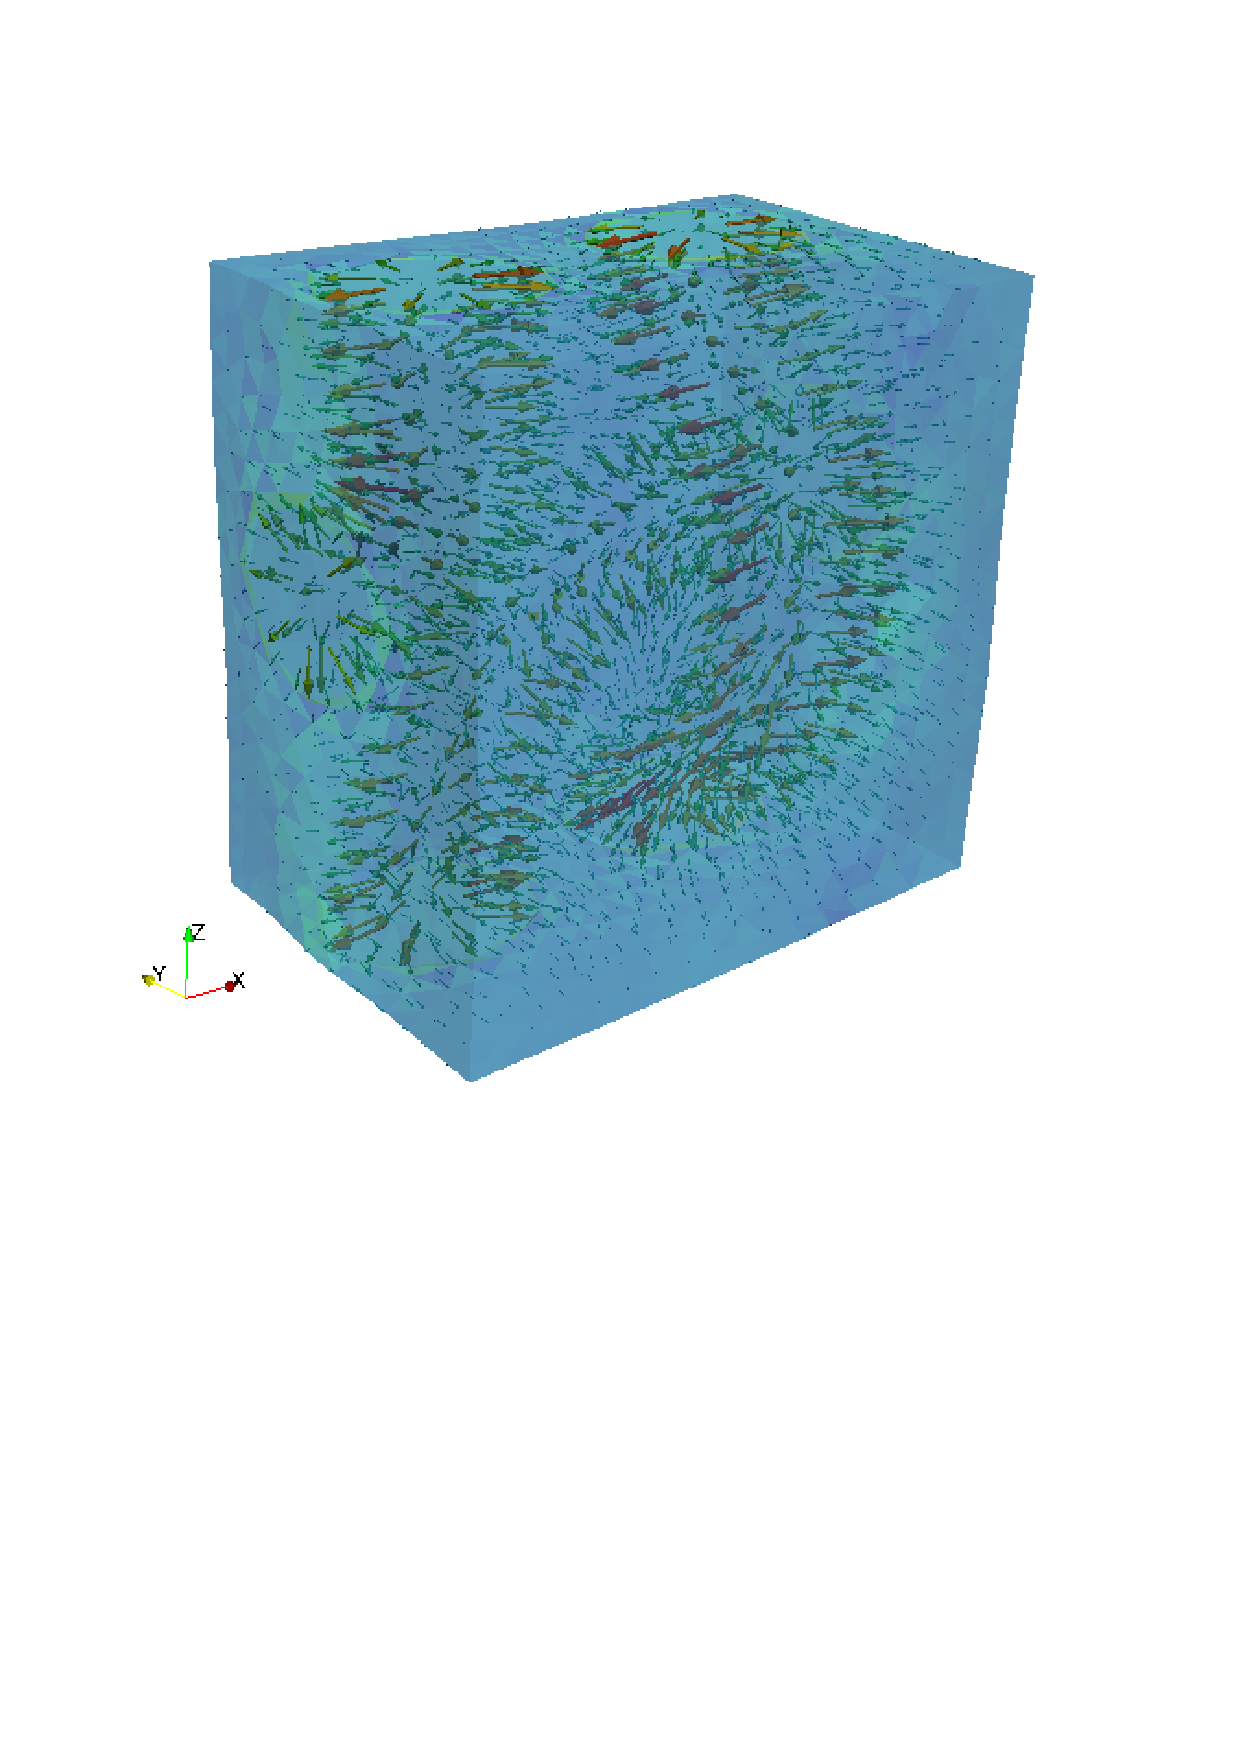
\includegraphics[width=0.5\linewidth]
        {\figDirHomPerfusion/steady_rs_00_u_M2_2}
        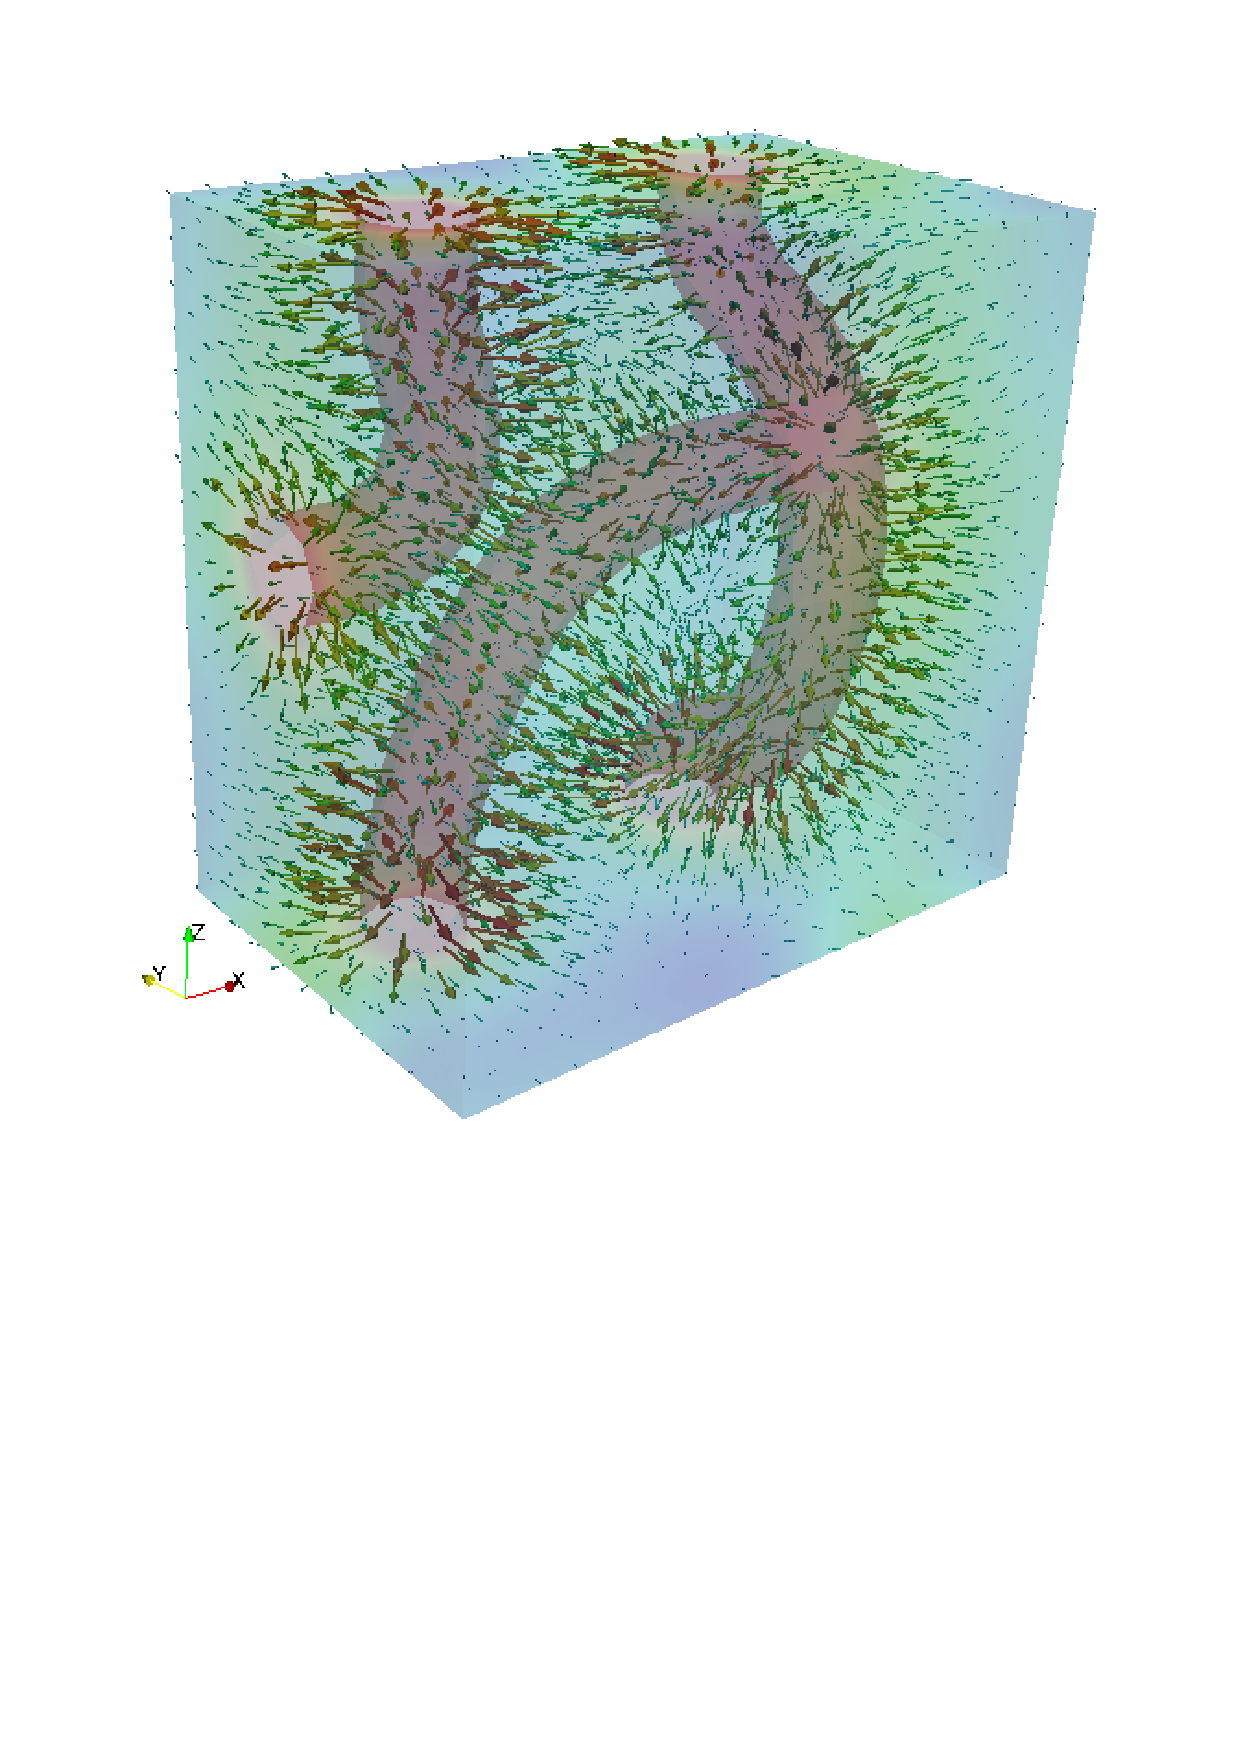
\includegraphics[width=0.5\linewidth]
        {\figDirHomPerfusion/steady_rs_00_p_M2_2}
      \end{center}
    \end{minipage}
  \end{center}
\end{frame}


\subsection{Microscopic Stress Recovery: Bones}

\begin{frame}
  \frametitle{Microscopic Stress Recovery: Bones}
  \begin{itemize}
  \item cortical bone: \emph{double porous medium}?
    \begin{itemize}
    \item macro-scale: a piece of compact bone (10 mm)
    \item meso-scale -- \blue{level 1} -- Haversian and Volkmann channels (100
      $\mu$m)
    \item micro-scale -- \blue{level 2} -- canaliculi, lacunae in ``solid
      matrix'' (1 $\mu$m)
    \end{itemize}
    \centerline{
      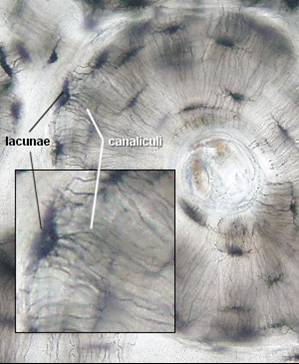
\includegraphics[width=0.14\linewidth]
      {\figDirHomBones//cortical-bone}
      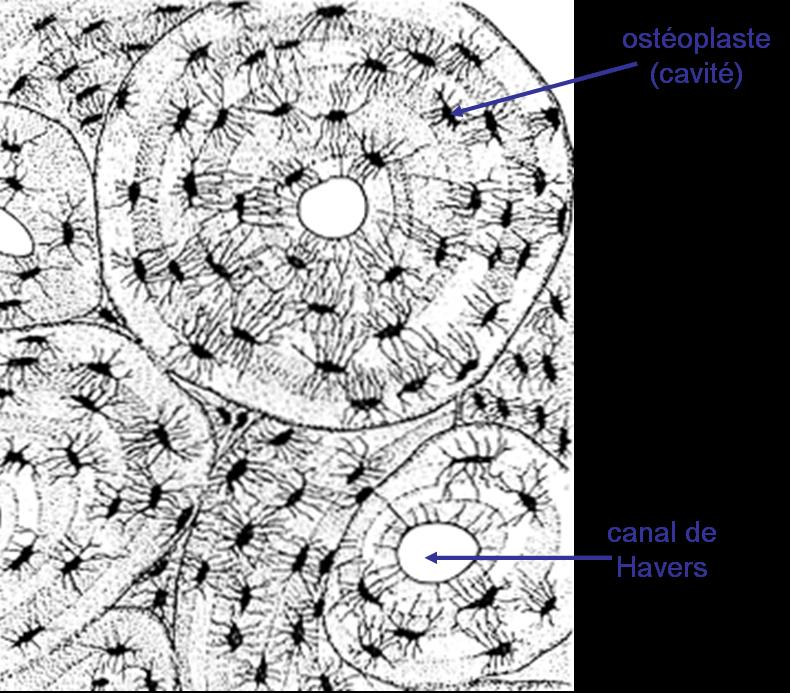
\includegraphics[width=0.2\linewidth]
      {\figDirHomBones//cortical-bone-sketch}
    }
  \item given macroscopic deformation and pressure, recover
    \begin{itemize}
    \item displacements $\ub^{\mic}$, pressure $p^{\mic}$
    \item micro-level $\ell^{\mu_1}$, sub-micro-level $\ell^{\mu_2}$ diffusion
    \end{itemize}
  \end{itemize}
  \begin{center}
    \begin{minipage}{0.32\linewidth}
      \scriptsize
      micro: various topologies, corrector functions \\
      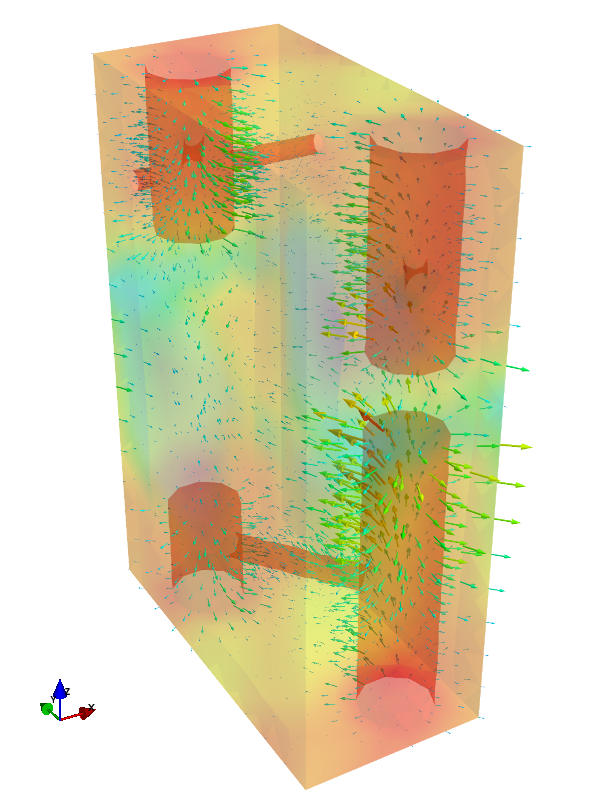
\includegraphics[width=0.48\linewidth]
      {\figDirHomBones/steady_rs_00_p_M1}
      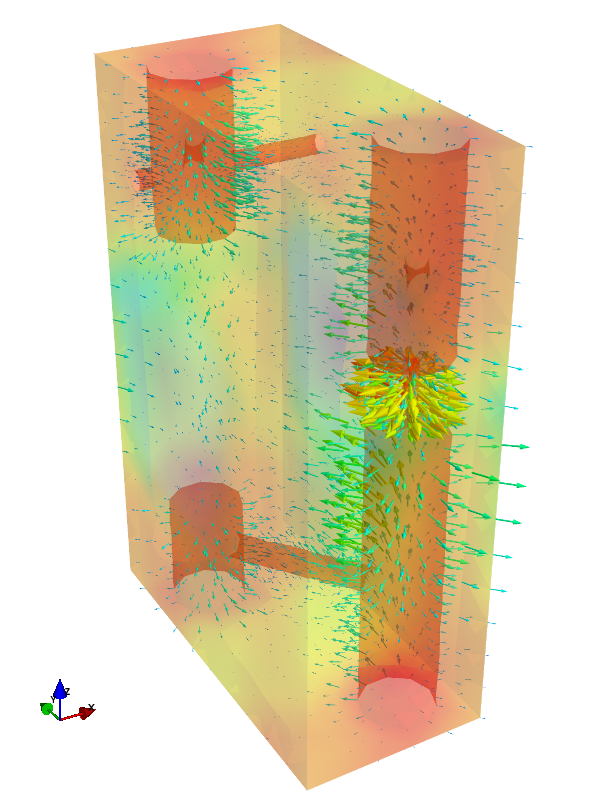
\includegraphics[width=0.48\linewidth]
      {\figDirHomBones/steady_rs_00_p_M2}
    \end{minipage}
    \hfill
    \begin{minipage}{0.17\linewidth}
      \scriptsize
      macro: compact bone segment \\
      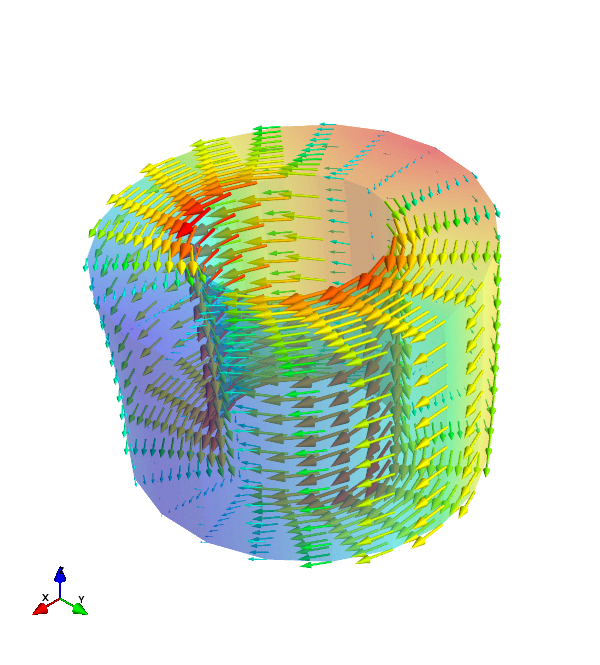
\includegraphics[width=0.9\linewidth]
      {\figDirHomBones/macro_t05_M2}
    \end{minipage}
    \hfill
    \begin{minipage}{0.45\linewidth}
      \scriptsize
      micro: recovery in a macro-point \\
      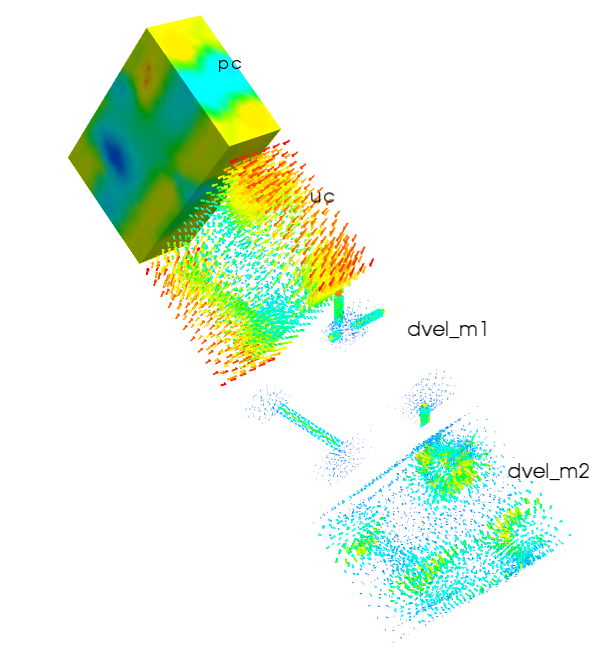
\includegraphics[width=0.48\linewidth]
      {\figDirHomBones/recovery_1999_200_M1}
      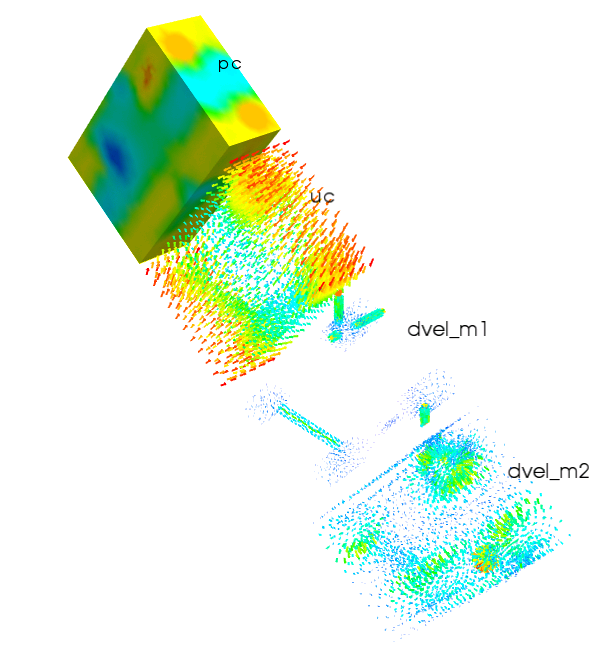
\includegraphics[width=0.48\linewidth]
      {\figDirHomBones/recovery_1999_200_M2}
    \end{minipage}
  \end{center}
\end{frame}


\section{Software}

\subsection*{}

\begin{frame}
  \frametitle{Software}
  \begin{flushleft}
    \begin{minipage}{0.5\linewidth}
      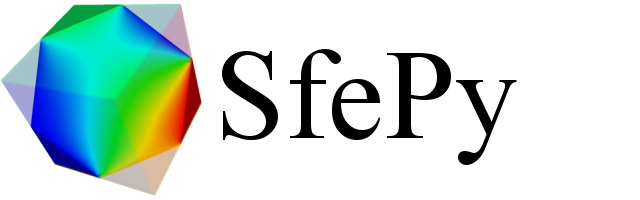
\includegraphics[width=\linewidth]{\figDirLogos/sfepy_logo_title}
    \end{minipage}
     = simple finite elements in Python
  \end{flushleft}
  \begin{itemize}
  \item general finite element analysis software
    \begin{itemize}
    \item solving systems of PDEs
    \end{itemize}
  \item<1-> BSD open-source license
  \item<1-> now multi-platform! (Linux, Mac OS X, Windows)
  \item<1-> available at
    \begin{itemize}
    \item 
      \href{http://sfepy.org}{\url{http://sfepy.org}} (developers)
      \begin{itemize}
      \item mailing lists, issue (bug) tracking
      \end{itemize}
    \item \href{http://sfepy.kme.zcu.cz}{\url{http://sfepy.kme.zcu.cz}}
      (project information)
    \end{itemize}
  \item work in progress\dots
  \end{itemize}
\end{frame}


\section{Conclusion}

\subsection*{}

\nocite{cimrman_et_al_2009:_sfepy}
\nocite{cimrman_rohan_2007:_modelling_parallel_diffusion}
\nocite{griso_rohan_2007:_homogenization_diffusion_deformation}
\nocite{rohan_2006:_modelling_large_deformation}
\nocite{rohan08:_homog_model_of_bone_poroel}
\nocite{rohan09:_multis_model_of_fluid_satur}

\begin{frame}[allowframebreaks]
  \frametitle{References}
  {\small The research was financially supported by the Grant Agency of the
    Czech Republic, project GA\v{C}R 106/09/0740, and the Czech Government
    project MSM 497751303.}

  \hrulefill
  \tiny
  \bibliography{bibliography}
\end{frame}

\end{document}
